\documentclass[sigconf]{acmart}

\usepackage{booktabs} % For formal tables


% Copyright
%\setcopyright{none}
%\setcopyright{acmcopyright}
%\setcopyright{acmlicensed}
\setcopyright{rightsretained}
%\setcopyright{usgov}
%\setcopyright{usgovmixed}
%\setcopyright{cagov}
%\setcopyright{cagovmixed}


% DOI
\acmDOI{10.475/123_4}

% ISBN
\acmISBN{123-4567-24-567/08/06}

%Conference
\acmConference[GECCO '17]{the Genetic and Evolutionary Computation Conference 2017}{July 15--19, 2017}{Berlin, Germany}
\acmYear{2017}
\copyrightyear{2017}

\acmPrice{15.00}


\begin{document}
\title{evospace-js: Asynchronous Pool-Based Execution of Heterogeneus Metaheuristics}
%\titlenote{Produces the permission block, and
%  copyright information}
\subtitle{Anonymized Version}
%\subtitlenote{The full version of the author's guide is available as
%  \texttt{acmart.pdf} document}


\author{Ben Trovato}
%\authornote{Dr.~Trovato insisted his name be first.}
\orcid{1234-5678-9012}
\affiliation{%
  \institution{Institute for Clarity in Documentation}
  \streetaddress{P.O. Box 1212}
  \city{Dublin} 
  \state{Ohio} 
  \postcode{43017-6221}
}
\email{trovato@corporation.com}

\author{G.K.M. Tobin}
%\authornote{The secretary disavows any knowledge of this author's actions.}
\affiliation{%
  \institution{Institute for Clarity in Documentation}
  \streetaddress{P.O. Box 1212}
  \city{Dublin} 
  \state{Ohio} 
  \postcode{43017-6221}
}
\email{webmaster@marysville-ohio.com}

\author{Lars Th{\o}rv{\"a}ld}
%\authornote{This author is the
%  one who did all the really hard work.}
\affiliation{%
  \institution{The Th{\o}rv{\"a}ld Group}
  \streetaddress{1 Th{\o}rv{\"a}ld Circle}
  \city{Hekla} 
  \country{Iceland}}
\email{larst@affiliation.org}

\author{Lawrence P. Leipuner}
\affiliation{
  \institution{Brookhaven Laboratories}
  \streetaddress{P.O. Box 5000}}
\email{lleipuner@researchlabs.org}



\begin{abstract}

This paper is part of an ever-growing effort in the field of EC to develop algorithms
following an opportunistic approach to computing, allowing the exploitation
of freely available services over the Internet or volunteer computing resources.
In this paper a version of the EvoSpace Model for the development of asynchronous
evolutionary algorithms is presented. The design follows an an event-driven 
architecture and asynchronous I/O. The server has been implemented as a Node.js
application using Redis as an in-memory data store. This high performance population
store is exposed to clients running population and nature-inspired metaheuristics
through a REST API. Additional capabilities where implemented in this version to
allow the logging of experiments where heterogeneous algorithms are executed in parallel.
These logs can then be transformed to other formats. As a case study
an hybrid global optimization algorithm has been implemented using an hybrid of
two algorithms: a PSO algorithm from the EvoloPy library and a GA using the DEAP framework.
The result was transformed to files compatible to the Comparing Continuous Optimizer platform
in order to use their post-processing code. Clients in this case have been developed in 
the Python language. The results from case study suggest that this software can yield
performance improvements and a viable platform to execute and compare asynchronous pool-based
metaheuristics.   
\end{abstract}

%
% The code below should be generated by the tool at
% http://dl.acm.org/ccs.cfm
% Please copy and paste the code instead of the example below. 
%
\begin{CCSXML}
<ccs2012>
<concept>
<concept_id>10010147.10010178.10010205.10010206</concept_id>
<concept_desc>Computing methodologies~Heuristic function construction</concept_desc>
<concept_significance>500</concept_significance>
</concept>
<concept>
<concept_id>10010147.10010178.10010205.10010207</concept_id>
<concept_desc>Computing methodologies~Bio Inspired Algorithms</concept_desc>
<concept_significance>500</concept_significance>
</concept>
</ccs2012>
\end{CCSXML}
\ccsdesc[500]{Computing methodologies~Heuristic function construction}
% We no longer use \terms command
%\terms{Theory}

\keywords{Nature-inspired metaheuristics, Distributed Evolutionary Algorithms}


\maketitle

\section{Introduction}
% Main Ideas:
%Why Paralel
A large body of work exists on the parallelization of EAs,
with techniques leveraging multiple CPU cores, many computing nodes, 
and GPUs \cite{muhlenbein1989parallel,cantu2000efficient,hofmann2013performance}. 
However, asynchronous EAs
\cite{Jini:FEA2000,alba2001analyzing,Jini:FEA2000,jj:2008:PPSN} have
started to become common only relatively
recently, in an effort to exploit computing resources available
through different Internet technologies, including cloud. In this work, we are
interested in those EAs following a pool-based approach,
where a collection of heterogeneous worker processes 
carry out population search tasks by collaborating through a shared
individual 
repository or population pool. We will refer to such algorithms 
as {\em Pool-based EAs} or PEAs, and highlight the fact that 
such systems are intrinsically parallel, distributed and asynchronous.

Pool-EAs differ from the closely related island model, 
mainly with regards to the responsibilities assigned to 
the server. When there is a server in the island model, it is 
responsible for the interaction and synchronization of 
all the populations.  In Pool-EAs, on the other hand, the population repository only 
receives stateless requests from isolated workers 
or clients. In this way, Pool-EAs are capable of using and leveraging an 
ad-hoc and ephemeral collaboration of computing resources. 

The platform presented in this paper is a new implementation 
of the EvoSpace model \cite{GValdez2015} in which 
workers asynchronously interact with the population 
pool by taking samples of the population 
to perform a local evolutionary search on the samples, 
to then return newly evolved solutions back to the pool. This is a
particular instance of a pool-based EA, which, as long as there is a
common population pool, leaves every other detail to particular
implementations. Other PEAs, for instance, might return only one
individual to the pool, or use it as a read-only resource, not
returning any member to it; the {\em frequency} with which resources
are taken or returned to the population are not set by the model
either, leaving it as a implementation or model-specific parameter. % I am giving here a general overview of PEAs, maybe it should be moved up with a few references? - JJ

The previous version % anonymized reference
was implemented using CherryPy, a basic HTTP 
server written in Python. This new version uses Node.js, an 
event-driven interpreter with a built-in event loop capable of
asynchronous I/O \cite{tilkov2010node}, that is 
running on the JavaSacript V8 engine. Node.js is used 
to optimize throughput and scalability of the server. %Actually you
                                %are using express, I think. You
                                %should talk about that - JJ
Additionaly to the  increased performance this version 
adds new functionality: In the former version workers could only
ask for random samples of a particular size, now clients 
can retrieve objects from the server ordered by a score. 
Designers can use this functionality to implement 
asynchronous versions of the Island Model or to force 
the retrieval of different objects in every request 
resembling a circular queue. Instead of using the JSON-RPC 
protocol the server functionality is now exposed as a RESTful 
Web Service. The server now keeps a log of the work performed 
by workers: The number of evaluations, the best solution in each 
generation (or iteration), parameters and algorithm used among others.
This log can later be used to compare the performance of 
the algorithm against others, for instance against 
algorithms using the COCO (COmparing Continuous Optimisers)
platform \cite{hansen2016coco}.
The aim of the evospace-js software is to provide 
researchers with a high performance platform in which 
they can execute pool-based algorithms using heterogeneous workers. 

The remainder of the paper proceeds as follows. Section \ref{sec:work} 
reviews related work. Afterwards, Section \ref{sec:evo} describes the
proposed EvoSpace implementation, the experimental work is presented in 
Section \ref{sec:experiments}. Finally, a summary and 
concluding remarks are given in Section \ref{sec:conclusions}.


\section{Related Work}
\label{sec:work}
There are two important practical issues faced by many EA systems, namely the size of the parameter 
space and the high computational cost when it is compared with mathematical programming or numerical techniques.
Concerning the latter, one approach to mitigate this issue is to use parallel or 
distributed implementations \cite{cantu-paz:migration-policies,duda2013gpu}.
For instance, Fern\'andez et al. \cite{nc} % articulo Paco, Gustavo y Leo publucado en Natural Computing}
uses the well-known Berkeley Open Infrastructure for Network Computing (BOINC) to distribute EA runs across a
heterogeneous network of volunteer computers using virtual machines. Another recent example is 
found in the FlexGP system developed by Sherry et al. \cite{sherry2012flex}. FlexGP is probably the first large scale GP system 
that runs on the cloud, using an Island model approach and implemented over Amazon EC2 with a 
socket-based client-server architecture.

Another approach to distributed EAs is the so called pool-based architecture. In general, a 
pool-based system employs a central repository (real or virtual) where the evolving population is stored.
Distributed clients interact with the pool, performing some or all of the basic EA processes 
(selection, genetic operators, survival). A representative work of this approach 
is that by Merelo et al. \cite{agajaj} implementing a JavaScript based PEA that distributes 
the evolutionary process over the web, providing the added advantage of not requiring the 
installation of additional software in each computing node.  Other similar cloud-based solutions 
are based on a global queue of tasks and a Map-Reduce implementation which normally handles failures 
by the re-execution of  tasks \cite{fazenda2012,di2013towards,FlexGP}. Using the BOINC 
volunteer platform  Smaoui et al. \cite{FekiNG09} uses work units that consist of a fitness 
evaluation task and multiple replicas  were produced and sent to different clients.

While using a distributed framework can ease the computational cost, it can also exacerbate the first issue mentioned above;
i.e., it increases the size of the algorithm parameter space, which makes parameter tuning a more difficult task.
The issue of optimal parametrization of EAs is a widely studied subject \cite{de2007parameter}, 
with many approaches in literature. For instance, one of the most successful approaches 
is the F-Racing and iterative F-Racing techniques \cite{lopez2011irace}. 
However, while such algorithms can find high performance parametrization, 
they require additional computational effort which can be too expensive in some applications
(even if they are more efficient than an exhaustive search).

\begin{figure}[!t]
    \centering
        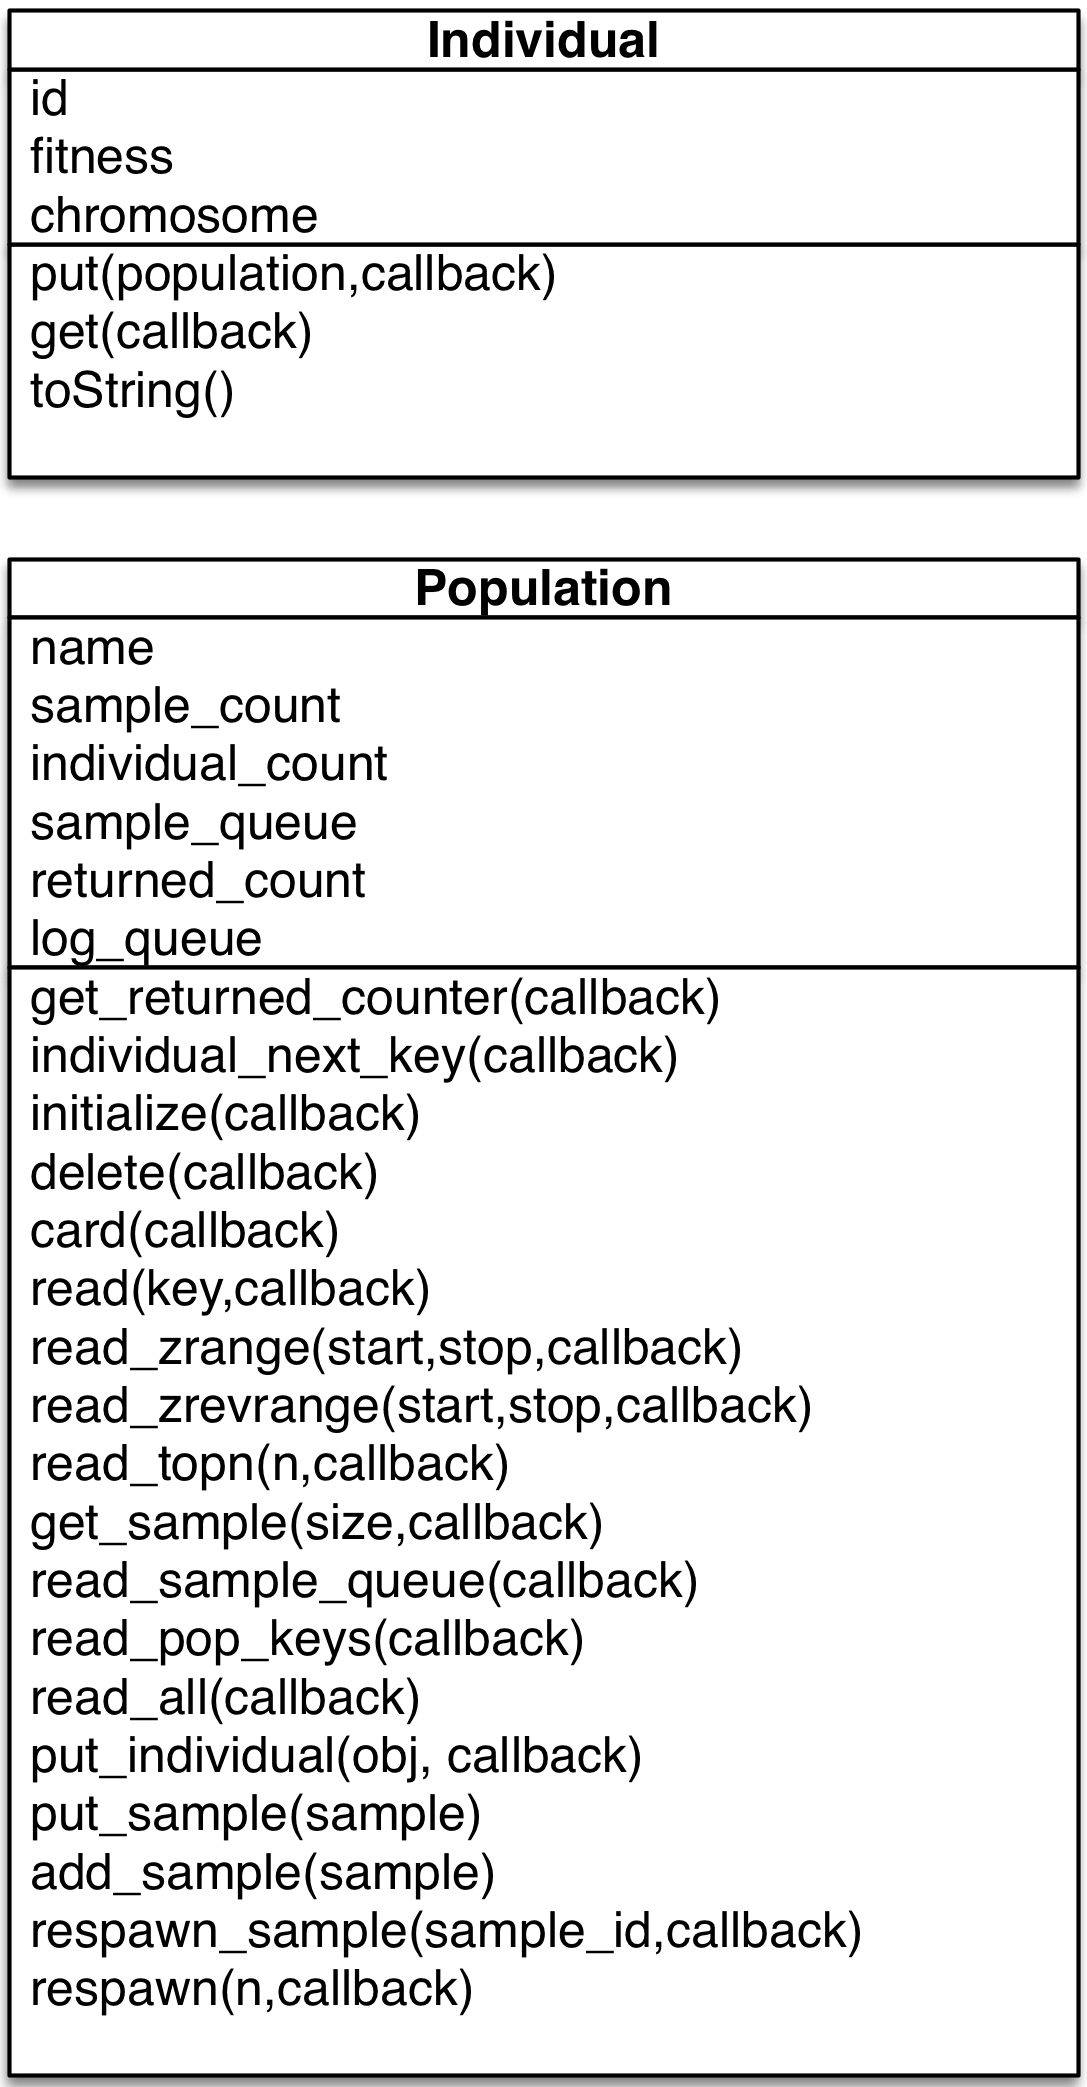
\includegraphics[width=2.5in]{img/classes.png}
    \caption{ UML Class diagram of the Population and Individual classes.}
    \label{fig:classes}
\end{figure}
%
\begin{figure*}[!t]
    \centering
        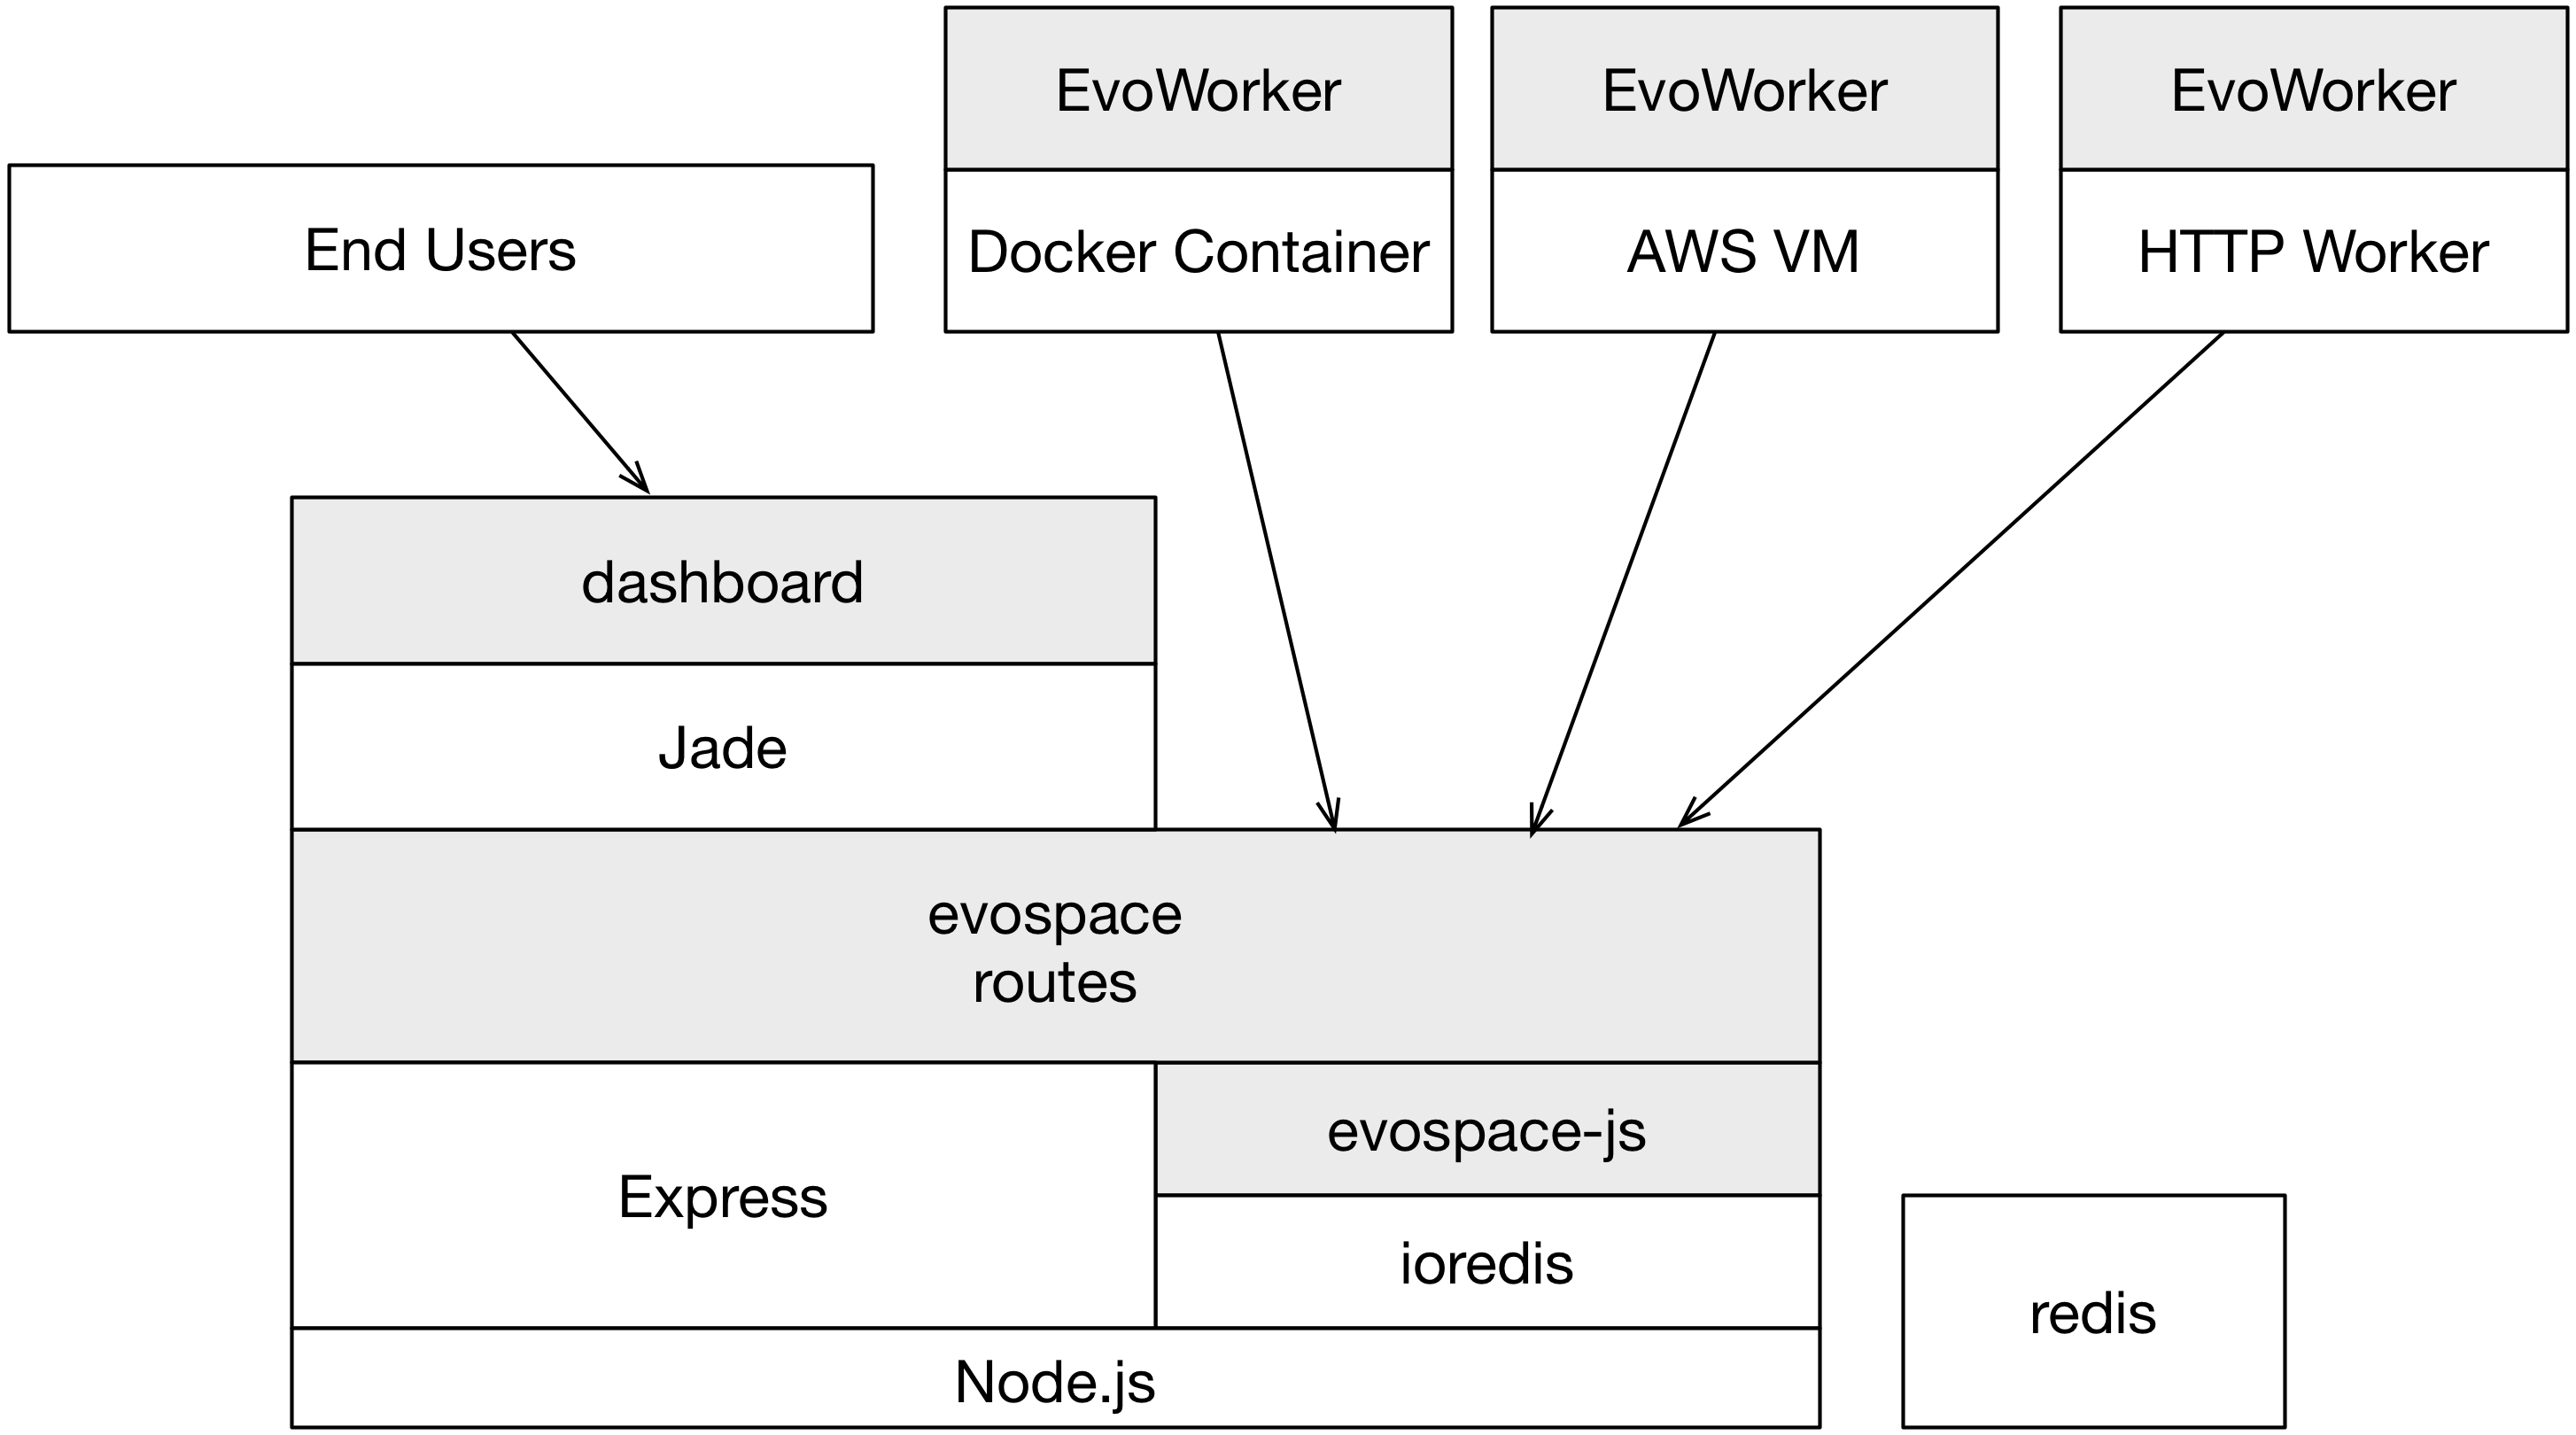
\includegraphics[width=5.4in]{img/evospace-js.png}
    \caption{ Stack diagram of the evospace-js framework components.}
    \label{fig:stack}
\end{figure*}

\section{evospace-js Implementation}
\label{sec:evo}
The main components of the EvoSpace framework are: the evospace-js 
population container, remote clients called EvoWorkers.
Each of these components are defined in the following subsections.

\subsection{evospace-js}
 \label{sec:evospace}
The evospace-js server provides a collection of REST methods  
to operate over a set of objects $ES$, which can be seen as the 
population. Multiple populations can be created and are 
distinguished by their name. Objects in each $ES$ 
can be selected, removed and replaced through the 
following endpoints:
\begin{enumerate}
    \item {\bf population\_name/initialize} 
    This is a {\tt POST} request used to create a new population.
    \item {\bf population\_name/individual} 
    This is a {\tt POST} request used to create and add a new object
    to a population. The object is defined in a JSON format, 
    and there is no restriction on its structure, only 
    the following properties are required: ``id'' this is an 
    integer and is generated if not present, ``fitness'' also defined 
    as a JSON object, the structure been specific to each application, 
    and finally a ``chromosome'' property again defined as
    a JavaScript object giving the internal representation of 
    the solution, by default a it defined as list of objects. 
    There is also an optional integer property called 
    ``score'' used when objects are going to be retieved in a certain order.
    \item {\bf population\_name/sample/n}
    This is a {\tt GET}  request used to take from the population a 
    sample of {\bf n} objects. These objects are removed from the 
    population and are no longer available
    to other requests until and only if they are put back. 
    Objects can be returned to the population 
    either by a {\tt PUT} sample request called from the same 
    client or by a Respawn request. The reason for 
    this is to avoid concurrently write conflicts and duplication of work.
    \item {\bf population\_name/sample}
    This is a {\tt POST} request used to put back a sample to the population.
    The new sample is sent in the request body as a JSON object. 
    If the client created new objects or 
    changed their original state, these objects replace the originals. 
    \item {\bf population\_name/respawn}
    This is a {\tt POST} request used to put back {\bf n} samples to their 
    original state. The number of samples is sent in the request body. 
\end{enumerate}
There are other secondary REST endpoints used to: select all objects in a 
population, select objects with scores with in a range, read the 
top {\tt n} objects according to a score and read the number of
objects currently on the population.      

The above methods were implemented first as JavaScript library 
with two classes: {\tt Individual} and {\tt Population} depicted 
in Figure~\ref{fig:classes} with calls to the Redis memory store 
through the {\bf ioredis} 
asynchronous library. In order to expose the library as a 
REST Web service endpoints were implemented using the Express HTTP framework. 
An optional dashboard type application, can be used to inspect 
the populations currently available on the server.


When a worker is putting back a sample, it can send 
an additional property called {\tt benchmark\_data }
to send supplementary information about the execution 
of the experiment.  This data can later be used to 
benchmark the performance of the algorithm. This 
data is again stored in redis as an ordered list, 
keeping a log for each experiment. Currently the JSON 
benchmark data structure contains the following details 
to later be used by the COCO platform: the algorithm identifier, 
parameters used, name , dimension, instance and optimal value 
of the function that is been optimized, worker and experiment 
identifiers and finally a list of details of each iteration 
or generation of the local execution. The details include:
the best solution and the function value, and the number of
function evaluations requiered. Depending on the application
other data could be recorded. The source code for the {\ss evospace-js}
server is in the following Github repository: 
\url{https://github.com/mariosky/evospace-js}.


\subsection{EvoWorkers}
\label{sec:evoworkers}
As we mentioned earlier, EvoWorkers are independent of 
the population store, and developers can implement them 
in any language that supports HTTP requests. To develop an 
EvoWorker, a programmer could just write the code needed to 
take a sample of the population and use this sample to 
replace the initial population of a local algorithm. 
Then after a certain number of iterations return the 
current population back to the server.

In this work, EvoWorkers were implemented in Python 
using two open source libraries of nature inspired optimization 
metaheuristics:  DEAP and EvoloPy. For each algorithm a 
python script was responsible for the initialization using 
the required parameters and setting up the initial population, 
then after some iterations, the current population and 
benchmark data is sent back to the server. EvoWorker 
scripts can run in Docker containers, by receiving 
the initial parameters as environment variables, and 
the script ends when it reaches a maximum number of samples.
The source code for the Python EvoWorkers
proposed in this work are on following Github repository: 
https://github.com/mariosky/EvoWorker.

\section{Experiments}
 \label{sec:experiments}



\section{Conclusions and Further Work}
\label{sec:conclusions}

% To be written

Future lines of work will focus on using other EA or meta-heuristic techniques, 
such as genetic programming or particle swarm optimization for having 
workers that are heterogeneous in more than one sense. RPSS could be
used in those cases where each algorithm has different sets of
parameters, but also to randomly select the technique used in each
node. Another interesting line of work is the dynamic adaptation of
parameters by measuring the diversity of each worker or returned
sample. This could be specially useful in cases where the random
parametrization technique seems to achieve bad results. 

\begin{acks}
This work has been supported in part by:  Ministerio espa\~{n}ol de
Econom\'{\i}a y Competitividad under project TIN2014-56494-C4-3-P
(UGR-EPHEMECH).
\end{acks}


\bibliographystyle{ACM-Reference-Format}
\bibliography{../bib/biblio,../bib/evospace-i,../bib/parameters,../bib/volunteer,../bib/geneura} 

\end{document}
